%\begin{figure}[!htpb]
%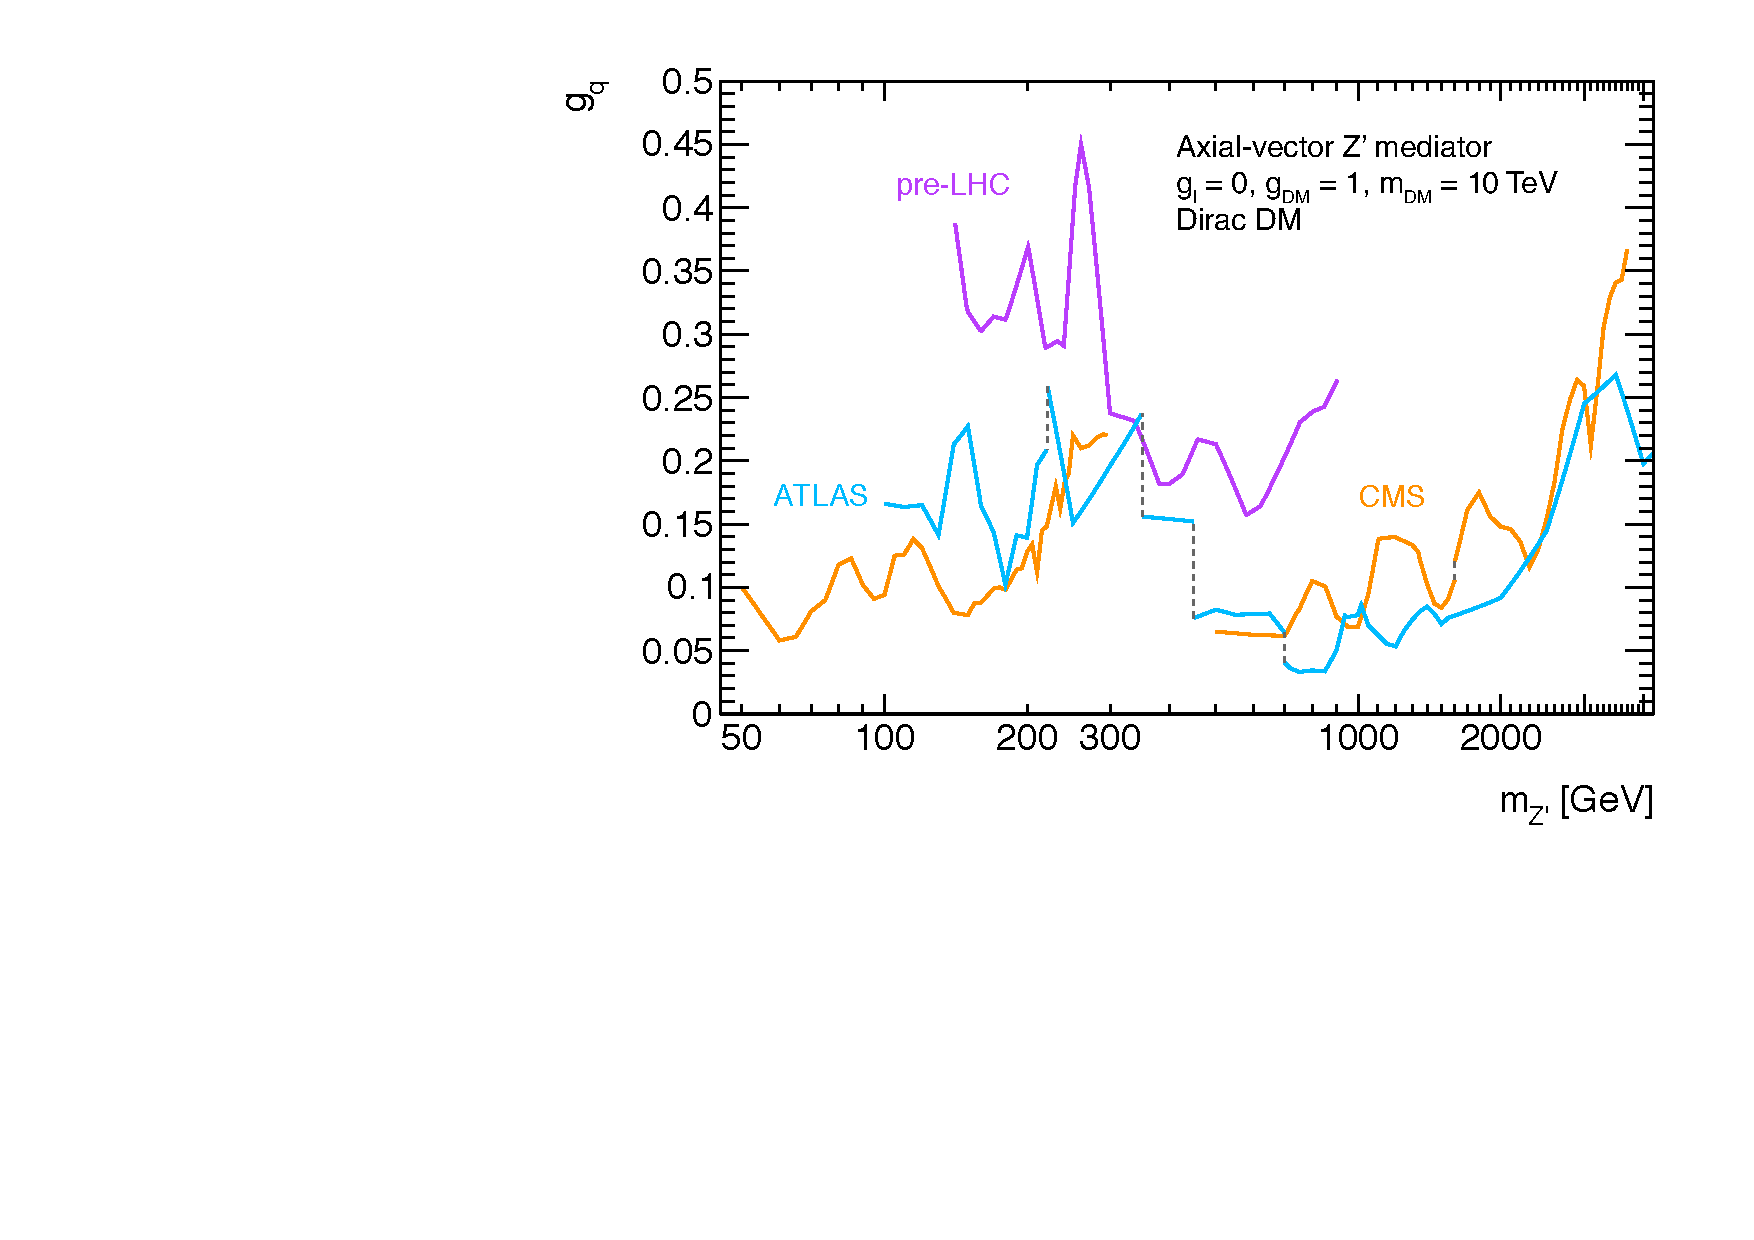
\includegraphics[width=\textwidth]{figures/CouplingMassPlot.pdf}
%\caption{

Summary of constraints from searches for narrow, light dijet
resonances from ATLAS and CMS available as of
July 2018, where discrete points are taken
from the coupling-mass limits on a simplified model mediated by an
axial--vector $Z^\prime$ coupling exclusively to quarks from the
searches mentioned in the text, and interpolated at the crossings.
Couplings above the lines are excluded at 95\% CL, up to the
values where larger couplings yield a resonance width larger than
10-15\% (roughly \gq $>$ 0.5). Abbreviation:\ DM, dark matter.
Pre-LHC constraints are extracted from Reference \citen{Dobrescu:2013coa},
while LHC constraints are taken from References \cite{Khachatryan:2016ecr,Aaboud:2018zba,
ATLAS:2016bvn,Sirunyan:2017nvi,Sirunyan:2018xlo,Aaboud:2018fzt,Aaboud:2017yvp}.

%}
%\label{fig:couplingmass}
%\end{figure}
